% The MEW nozzle in the round, with heat: a short results note for Murat Kilic.
% Build: make -C paper/mew_axi   (figures: make -C paper/mew_axi figs, after the runs)
\documentclass[10pt,a4paper]{article}
\usepackage[T1]{fontenc}
\usepackage[utf8]{inputenc}
\usepackage{sourceserifpro}
\usepackage{sourcesanspro}
\renewcommand{\familydefault}{\rmdefault}
\usepackage[a4paper,margin=2.1cm,top=1.6cm,bottom=1.8cm]{geometry}
\usepackage{graphicx}
\usepackage{booktabs}
\usepackage{tabularx}
\usepackage{array}
\usepackage{microtype}
\usepackage[mode=text]{siunitx}
\usepackage{xcolor}
\usepackage{enumitem}
\usepackage{titlesec}
\usepackage[font={small,sf},labelfont={bf,sf},labelsep=period,skip=4pt]{caption}
\usepackage[colorlinks=true,linkcolor=melt,urlcolor=melt]{hyperref}

\definecolor{melt}{HTML}{2A78D6}
\definecolor{inktwo}{HTML}{4F4E4A}
\definecolor{inkthree}{HTML}{807F79}

\titleformat{\section}{\sffamily\bfseries\large}{\thesection}{0.6em}{}
\titlespacing*{\section}{0pt}{10pt}{4pt}
\titleformat{\subsection}{\sffamily\bfseries\normalsize}{\thesubsection}{0.6em}{}
\titlespacing*{\subsection}{0pt}{7pt}{2pt}
\setlength{\parskip}{3pt}
\setlength{\parindent}{0pt}
\setlist{nosep,leftmargin=1.2em,topsep=2pt}
\renewcommand{\arraystretch}{1.15}
\newcolumntype{L}{>{\raggedright\arraybackslash}X}

\hypersetup{pdftitle={The MEW nozzle in the round, with heat},pdfauthor={Alessandro De Rosis}}

\begin{document}

{\sffamily\footnotesize\color{inkthree}M3LB \textperiodcentered{} lattice Boltzmann \textperiodcentered{} round-nozzle (r--z) model\hfill 7 November 2026\par}
\vspace{6pt}
{\sffamily\bfseries\LARGE The MEW nozzle in the round, with heat\par}
\vspace{3pt}
{\sffamily\large\color{inktwo}What decides whether the melt reaches the collector, for the set-up of Ju, Omar, Mirihanage and Kilic\par}
\vspace{3pt}
{\small Alessandro De Rosis\par}
\vspace{8pt}

\textbf{Summary.} The notes of 3 and 5 November modelled the nozzle as a planar slice, with the melt held at
\qty{120}{\celsius}. Here the nozzle is round: the model uses its axial symmetry, so the melt's surface has
both of its curvatures, which a planar slice lacks and a Taylor cone needs. The melt can also cool. The set-up is
otherwise the same: PCL at \qty{820}{\pascal\second}, fed at \qty{0.0208}{\cubic\milli\metre\per\second}
through a \qty{0.4}{\milli\metre} nozzle \qty{5.5}{\milli\metre} above the collector, at \qty{6.5}{\kilo\volt}.
Four results:
\begin{itemize}
  \item \textbf{Held at \qty{120}{\celsius}}, the field draws the drop into a column that reaches the collector
    after \qty{15.8}{\second} on \qty{50}{\micro\metre} cells and \qty{9.8}{\second} on \qty{25}{\micro\metre}
    cells. The time is not converged and cannot be: the model's perfectly conducting tip sharpens without limit
    on finer cells. It is not a prediction, here or in the planar and 3-D runs.
  \item \textbf{Allowed to cool}, with estimated values for the air (\qty{25}{\celsius}) and for the heat it
    draws from the surface (\qty{90}{\watt\per\square\metre\per\kelvin}), the drop's lower end falls below
    \qty{40}{\celsius} after \qty{23}{\second} and starts to crystallise. The drop then stops about
    \qty{3.5}{\milli\metre} above the collector while melt piles up at the tip,
    \qty{1.34}{\cubic\milli\metre} within \qty{1}{\milli\metre} of it after \qty{150}{\second}. That is
    oozing, not a jet, and it holds on finer cells.
  \item \textbf{The air at the tip decides between the two.} With the air at \qty{35}{\celsius} the drop
    still stops; at 40 and \qty{50}{\celsius} it reaches the collector after 31 and \qty{28}{\second}. Once
    the drop cools, the field, the surface tension and the shape of the electrodes change little.
  \item \textbf{The printer does make fibres}, so something at its tip must differ from these estimates: most
    simply, the air there is warmer than \qty{25}{\celsius}, or PCL crystallises lower than assumed, or the
    jet is started in a way the model leaves out. Four questions would settle it
    (Section~\ref{sec:questions}).
\end{itemize}

\section{Model and set-up}

\begin{tabularx}{\textwidth}{@{}>{\leavevmode\sffamily\small\color{inktwo}}p{2.2cm}L@{}}
\toprule
Geometry & The round nozzle, through its axial symmetry: a two-dimensional model in radius and height
  (r--z) that keeps the curvature around the axis a planar slice loses. A \qty{0.4}{\milli\metre} bore and an
  assumed \qty{1.0}{\milli\metre} tip face, \qty{5.5}{\milli\metre} above a grounded collector at
  \qty{6.5}{\kilo\volt}. The collector is at rest, since a moving plate is not axially symmetric; nothing after
  contact is used. \\
Melt & PCL at \qty{120}{\celsius}: \qty{820}{\pascal\second} (measured),
  \qty{1080}{\kilo\gram\per\cubic\metre}, surface tension \qty{0.03}{\newton\per\metre} (nominal). The whole
  drop conducts, as the estimated conductivity implies (note of 5 November), so the planar model's conducting
  depth is gone. \\
Feed & \qty{0.0208}{\cubic\milli\metre\per\second}, delivered exactly in volume. \\
Field & The potential in the air, with the melt at the nozzle's potential. The air is a cylinder
  \qty{4}{\milli\metre} in radius whose side and top carry no field; a long needle and a plate across the top
  were run as checks (Section~\ref{sec:decides}). \\
Heat & New. The melt conducts and carries heat (conductivity \qty{0.20}{\watt\per\metre\per\kelvin}, heat
  capacity \qty{2000}{\joule\per\kilo\gram\per\kelvin}, both nominal) and loses it through its surface to air
  at \qty{25}{\celsius}, at \qty{90}{\watt\per\square\metre\per\kelvin} (nominal: natural convection and
  radiation). Nozzle at \qty{120}{\celsius}, collector at \qty{22}{\celsius}. The viscosity rises as the melt
  cools (Arrhenius, \qty{31.3}{\kilo\joule\per\mole} from the literature: 8 times its \qty{120}{\celsius}
  value at \qty{50}{\celsius}, 17 times at \qty{30}{\celsius}), and between 40 and \qty{30}{\celsius} the melt
  crystallises, modelled as a drag that brings it to rest. \\
Grid & \qty{50}{\micro\metre} cells, with \qty{25}{\micro\metre} as a check; \qty{57}{\micro\second} steps.
  A free-surface lattice Boltzmann model of the melt (the air is not simulated), and finite volumes for the
  potential and the temperature on the same cells. \\
\bottomrule
\end{tabularx}

\smallskip
Matched to the experiment, as before: the capillary number of the feed (4.5), the Bond number (0.014) and the
ratio of electric to capillary pressure (62).

\section{Results}

\subsection{\texorpdfstring{Held at 120\,°C}{Held at 120 °C}: a column, but no converged time}
With the melt held at \qty{120}{\celsius}, as in the planar and 3-D runs, the field draws the drop into a
column (Fig.~\ref{fig:heat}a, blue; Fig.~\ref{fig:heat}b) that reaches the collector after
\qty{15.8}{\second} on \qty{50}{\micro\metre} cells and \qty{9.8}{\second} on \qty{25}{\micro\metre} cells.
The finer cells resolve a sharper tip: around \qty{9}{\second} the electric pull there is about 42 times the
capillary pressure of the bore, against 6 on the coarser cells, and the drop is \qty{5}{\milli\metre} above
the collector after \qty{3.2}{\second} rather than \qty{3.8}{\second}. Nothing in the model limits a perfect
conductor's tip: no current leaves with the melt, and the air does not break down, although the field at the
drop, 11 to \qty{43}{\kilo\volt\per\milli\metre} as it approaches, is far above the roughly
\qty{3}{\kilo\volt\per\milli\metre} at which air breaks down. The contact time is therefore not a
prediction. With the field off the drop sags under its own weight, is
\qty{1.78}{\milli\metre} above the collector after \qty{150}{\second}, and touches after
\qty{195}{\second}. The planar model, with its earlier surface treatment, touched after \qty{91}{\second}: a
planar drop holds less melt for its outline.

\begin{figure}[t]
  \centering
  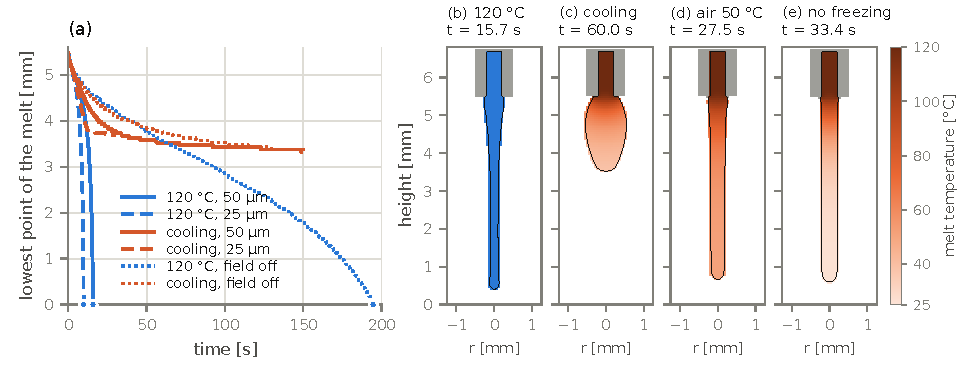
\includegraphics[width=\textwidth]{fig/fig1_heat.pdf}
  \caption{(a) Height of the lowest point of the melt against time, held at \qty{120}{\celsius} (blue) and
    allowed to cool (orange), on \qty{50}{\micro\metre} (solid) and \qty{25}{\micro\metre} cells (dashed),
    and with the field off (dotted, \qty{50}{\micro\metre}). Dots mark first contact with the collector.
    (b--e) The drop, mirrored about the axis, coloured by temperature (blue: held at \qty{120}{\celsius}),
    with the nozzle in grey: (b) held at \qty{120}{\celsius}, just before contact; (c) cooling, stopped;
    (d) cooling in air at \qty{50}{\celsius} and (e) without the freezing drag, both just before contact.
    The two cooling runs with the field on in (a) cap the viscosity's rise at 6-fold, the rest at 24-fold;
    under the two caps the nominal run stays within a cell from 10 to \qty{60}{\second}.}
  \label{fig:heat}
\end{figure}

\subsection{Allowed to cool: the drop stops and oozes}
With heat (Fig.~\ref{fig:heat}a, orange; Fig.~\ref{fig:heat}c), the melt leaving the bore cools from its
surface. Its lower end falls below \qty{45}{\celsius} after \qty{18}{\second} and below \qty{40}{\celsius}
after \qty{23}{\second}, enters the freezing band and stiffens, and the drop all but stops:
\qty{3.53}{\milli\metre} above the collector after \qty{60}{\second}, \qty{3.38}{\milli\metre} after
\qty{150}{\second}. It widens instead, to \qty{1.64}{\milli\metre} across, and the melt piles up at the tip,
\qty{1.34}{\cubic\milli\metre} within \qty{1}{\milli\metre} of it after \qty{150}{\second}, while the melt
below the tip averages \qty{51}{\celsius}. On \qty{25}{\micro\metre} cells, taken to \qty{30}{\second}, the
drop is \qty{3.69}{\milli\metre} up after \qty{28}{\second} against \qty{3.78}{\milli\metre} on
\qty{50}{\micro\metre} cells, \qty{0.77}{\milli\metre} wide against \qty{0.76}{\milli\metre}, with
\qty{6}{\percent} less melt at the tip. Unlike the column, this result holds on the finer cells.

With the field off the cooling drop comes down more slowly but stops at the same height
(Fig.~\ref{fig:decides}c): \qty{0.25}{\milli\metre} higher after \qty{60}{\second}, at the same
\qty{3.43}{\milli\metre} after \qty{120}{\second}, and \qty{3.33}{\milli\metre} up after \qty{150}{\second}
with \qty{1.54}{\cubic\milli\metre} at the tip. Letting the melt ooze for \qty{60}{\second} and then
switching the field on does not make a jet: after \qty{120}{\second} the drop is one cell lower than with the
field off (3.38 against \qty{3.43}{\milli\metre}) and holds less at the tip (1.20 against
\qty{1.32}{\cubic\milli\metre}), with a field of about \qty{10}{\kilo\volt\per\milli\metre} where it is
strongest on its surface.
Once the drop has cooled, the field barely moves it.

\subsection{What decides it}\label{sec:decides}
Figure~\ref{fig:decides} changes the estimates one at a time. The air at the tip decides between the two
outcomes (Fig.~\ref{fig:decides}a). At \qty{35}{\celsius} the drop still stops, \qty{2.7}{\milli\metre}
up; at 40 and \qty{50}{\celsius} its end does not reach the freezing band, and it reaches the collector after
30.5 and \qty{28.1}{\second} as a cold column (Fig.~\ref{fig:heat}d). The drop stops when the air can cool its
end into the band. Without the freezing drag it also reaches the collector, after \qty{34.3}{\second}
(Fig.~\ref{fig:heat}e): the rising viscosity slows the melt but does not stop it. The cooling sets where it
stops (Fig.~\ref{fig:decides}b). At 30, 90 and \qty{300}{\watt\per\square\metre\per\kelvin} the drop stops
1.9, 3.5 and \qty{4.3}{\milli\metre} above the collector, holding 0.47, 0.75 and
\qty{1.17}{\cubic\milli\metre} within \qty{1}{\milli\metre} of the tip after \qty{60}{\second}: the stronger
the cooling, the sooner the end freezes and the more melt is held at the tip. A freezing band of 20 to
\qty{30}{\celsius} in place of 30 to \qty{40}{\celsius} lets the drop down to \qty{2.6}{\milli\metre}.
Surface tension \qty{20}{\percent} higher or lower leaves the drop in the same cell and the melt at the tip
within \qty{0.001}{\cubic\milli\metre}.

The electrodes matter less. Held at \qty{120}{\celsius}, in a box \qty{8}{\milli\metre} in radius, a long needle
(\qty{10}{\milli\metre} into the box) touches after \qty{15.1}{\second}, and a plate at the nozzle's potential
across the top, \qty{5}{\milli\metre} up the nozzle, after \qty{18.2}{\second}, against \qty{15.8}{\second}
in the default box: a pull at the tip \qty{35}{\percent} weaker delays contact by 15 to \qty{20}{\percent}.

\begin{figure}[t]
  \centering
  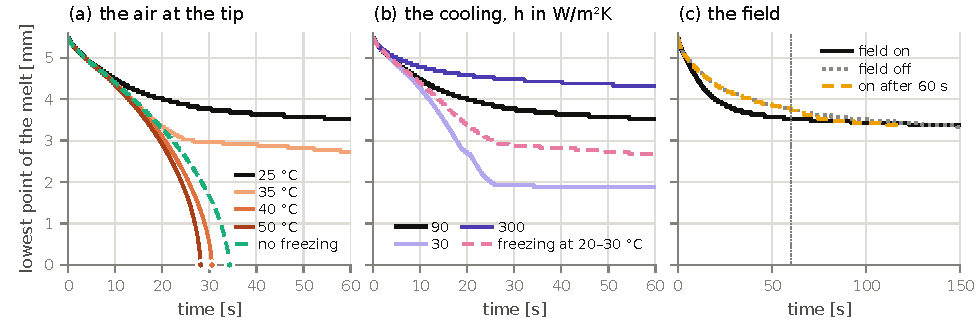
\includegraphics[width=\textwidth]{fig/fig2_decides.pdf}
  \caption{What decides it, on \qty{50}{\micro\metre} cells: the lowest point of the melt against time,
    changing one estimate at a time. Black is the nominal run (air at \qty{25}{\celsius},
    \qty{90}{\watt\per\square\metre\per\kelvin}, freezing at 30 to \qty{40}{\celsius}); dots mark first
    contact. (a) The air at the tip, and the run without the freezing drag. (b) The heat drawn from the
    surface, and a lower freezing band. (c) The field off, and switched on after \qty{60}{\second} (dotted
    line). The field-on run in (c) caps the viscosity's rise at 6-fold, the others at 24-fold.}
  \label{fig:decides}
\end{figure}

\section{What the model leaves out}
\textbf{The jet}: the preprint's fibres are 9.5 to \qty{22}{\micro\metre} across, below the finest cells
that can be afforded (\qty{25}{\micro\metre}), so the model resolves what gathers under the tip and nothing
that leaves it. \textbf{Charge and current}: the melt is a perfect conductor, no current leaves with it, and
the air does not break down. \textbf{The moving collector}: at rest, so nothing after contact is used.
\textbf{Crystallisation} is a drag switched on below a temperature band, with no kinetics and no latent
heat; the heat released as the melt crystallises would slow its end through the band.
\textbf{The heat values}: the heat drawn from the surface, the air's temperature, the conductivity and heat
capacity, the freezing band and the activation energy are all estimates.

\section{How far to trust it}

\begin{tabularx}{\textwidth}{@{}>{\raggedright\arraybackslash\sffamily\small}p{4.3cm}L@{}}
\toprule
Against the 3-D run of 6 November (held at \qty{120}{\celsius}, its own settings) &
  In a cylinder inscribed in its square box the column reaches \qty{0.5}{\milli\metre} above the collector
  after \qty{31.1}{\second}, against \qty{32.4}{\second} in 3-D, and the melt between tip and collector
  agrees to \qty{0.09}{\percent} over 1 to \qty{32}{\second}; in a cylinder of the same area,
  \qty{27.2}{\second}, the box's shape moving the field at the tip. \qty{7.6}{\minute} of computing against
  \qty{6.0}{\hour}. \\
Cell size, 50 and \qty{25}{\micro\metre} &
  Cooling: \qty{3.69}{\milli\metre} against \qty{3.78}{\milli\metre} after \qty{28}{\second}. Held at
  \qty{120}{\celsius}: contact after 9.8 and \qty{15.8}{\second}, not converged. \\
The model's own viscosity setting &
  Contact (\qty{120}{\celsius}) after 15.45, 15.69 and \qty{15.80}{\second} as it goes from 1/2 to 1/4 to
  1/6, against \qty{16.07}{\second} extrapolated: about \qty{2}{\percent}. \\
Flow, field and heat against exact solutions &
  Laplace's law for a sphere, \qty{1.0}{\percent} high at 8 cells and \qty{0.03}{\percent} at 16; pipe flow,
  second order; a drop relaxing to a sphere at 0.98 to 0.99 of the exact rate. A conducting sphere's field
  to \qty{3}{\percent} in amplitude, with a \qty{7}{\percent} cell-to-cell scatter from its stepped surface;
  coaxial electrodes, second order.
  Conduction in a cylinder to \qty{0.01}{\percent} at 32 cells; a sphere's heat loss \qtyrange{1.0}{1.2}{\percent}
  high. \\
Surface stiffness &
  Under a gentle electric pull the surface now deflects 4 to \qty{6}{\percent} too far (planar test); before
  the improved curvature used here it deflected 9 to \qty{20}{\percent} too little. \\
Mass &
  The fed melt is accounted for to \num{3e-5} after the first \qty{2}{\second} (\num{1.4e-5} on
  \qty{25}{\micro\metre} cells); to \num{2.3e-4} at the viscosity setting 1/2, and to \num{1.2e-3} in the
  comparison with 3-D, which uses that setting and the 3-D run's others. \\
\bottomrule
\end{tabularx}

\section{Questions for the experiment}\label{sec:questions}
\begin{enumerate}
  \item What is the air temperature a few millimetres below the tip while printing? A thermocouple would do.
    The model's answer changes between 35 and \qty{40}{\celsius}.
  \item After the voltage is switched on, does a jet start by itself, and after how long? If it needs help,
    how is it started?
  \item Is there a DSC trace of this PCL cooling at a few kelvin per second (the model's drop end averages
    about \qty{3.4}{\kelvin\per\second} from 120 to \qty{40}{\celsius})? Its crystallisation onset sets the
    band, 30 to \qty{40}{\celsius} here, and its latent heat is missing from the model.
  \item Could the viscosity data at 90, 100 and \qty{110}{\celsius} be shared? They would replace the
    activation energy taken from the literature.
\end{enumerate}

\vfill
{\footnotesize\color{inkthree}\sffamily M3LB (\href{https://github.com/alexderosis/M3LB}{github.com/alexderosis/M3LB},
branch \texttt{electrowriting}): \texttt{demonstrator/mew\_axi} with \texttt{-heat}, adding \texttt{-nu 0.0416666667}
for the 24-fold viscosity cap (the default, 1/6, caps at 6); \texttt{-Tair 35}, \texttt{40},
\texttt{50}; \texttt{-nofreeze}; \texttt{-h 30}, \texttt{300}; \texttt{-Tfreeze 20}; \texttt{-gamma 0.024},
\texttt{0.036}; \texttt{-nofield}; \texttt{-fieldon 60}. Electrodes \texttt{-W 8 -up 10} and
\texttt{-W 8 -up 5 -plateR 8}; \qty{25}{\micro\metre} cells \texttt{-R 8}; against 3-D \texttt{-W 2} (or
\texttt{2.26}) \texttt{-equip -lc 5 -nu 0.5 -nogeom -feed 0.02159}. Series and logs in
\texttt{results/mew\_axi}.\par}

\end{document}
